\documentclass[]{article}
\usepackage{lmodern}
\usepackage{amssymb,amsmath}
\usepackage{ifxetex,ifluatex}
\usepackage{fixltx2e} % provides \textsubscript
\ifnum 0\ifxetex 1\fi\ifluatex 1\fi=0 % if pdftex
  \usepackage[T1]{fontenc}
  \usepackage[utf8]{inputenc}
\else % if luatex or xelatex
  \ifxetex
    \usepackage{mathspec}
  \else
    \usepackage{fontspec}
  \fi
  \defaultfontfeatures{Ligatures=TeX,Scale=MatchLowercase}
\fi
% use upquote if available, for straight quotes in verbatim environments
\IfFileExists{upquote.sty}{\usepackage{upquote}}{}
% use microtype if available
\IfFileExists{microtype.sty}{%
\usepackage{microtype}
\UseMicrotypeSet[protrusion]{basicmath} % disable protrusion for tt fonts
}{}
\usepackage[margin=1in]{geometry}
\usepackage{hyperref}
\hypersetup{unicode=true,
            pdftitle={ActiveDriverWGS},
            pdfauthor={Helen Zhu, Dr.~Juri Reimand},
            pdfborder={0 0 0},
            breaklinks=true}
\urlstyle{same}  % don't use monospace font for urls
\usepackage{graphicx,grffile}
\makeatletter
\def\maxwidth{\ifdim\Gin@nat@width>\linewidth\linewidth\else\Gin@nat@width\fi}
\def\maxheight{\ifdim\Gin@nat@height>\textheight\textheight\else\Gin@nat@height\fi}
\makeatother
% Scale images if necessary, so that they will not overflow the page
% margins by default, and it is still possible to overwrite the defaults
% using explicit options in \includegraphics[width, height, ...]{}
\setkeys{Gin}{width=\maxwidth,height=\maxheight,keepaspectratio}
\IfFileExists{parskip.sty}{%
\usepackage{parskip}
}{% else
\setlength{\parindent}{0pt}
\setlength{\parskip}{6pt plus 2pt minus 1pt}
}
\setlength{\emergencystretch}{3em}  % prevent overfull lines
\providecommand{\tightlist}{%
  \setlength{\itemsep}{0pt}\setlength{\parskip}{0pt}}
\setcounter{secnumdepth}{5}
% Redefines (sub)paragraphs to behave more like sections
\ifx\paragraph\undefined\else
\let\oldparagraph\paragraph
\renewcommand{\paragraph}[1]{\oldparagraph{#1}\mbox{}}
\fi
\ifx\subparagraph\undefined\else
\let\oldsubparagraph\subparagraph
\renewcommand{\subparagraph}[1]{\oldsubparagraph{#1}\mbox{}}
\fi

%%% Use protect on footnotes to avoid problems with footnotes in titles
\let\rmarkdownfootnote\footnote%
\def\footnote{\protect\rmarkdownfootnote}

%%% Change title format to be more compact
\usepackage{titling}

% Create subtitle command for use in maketitle
\newcommand{\subtitle}[1]{
  \posttitle{
    \begin{center}\large#1\end{center}
    }
}

\setlength{\droptitle}{-2em}

  \title{ActiveDriverWGS}
    \pretitle{\vspace{\droptitle}\centering\huge}
  \posttitle{\par}
    \author{Helen Zhu, Dr.~Juri Reimand}
    \preauthor{\centering\large\emph}
  \postauthor{\par}
      \predate{\centering\large\emph}
  \postdate{\par}
    \date{2019-01-29}


\begin{document}
\maketitle

\section{Introduction}\label{introduction}

Cancer is driven by somatic mutations. A few of these mutations confer a
survival advantage to the tumour (drivers) while most mutations play a
passive role in tumour development (passengers). Most driver mutations
up to this point have been discovered in protein coding genes in whole
exome sequencing datasets. Yet, as whole genome sequencing datasets grow
and become the standard, novel methods are required to detect driver
mutations in the vast noncoding regulatory genome. Here, we present our
solution to this challenge, ActiveDriverWGS.

\subsubsection{The ActiveDriverWGS
Model}\label{the-activedriverwgs-model}

ActiveDriverWGS analyzes the mutational burden of \textbf{SNVs and short
indels} (less than 50bps) in functionally defined \textbf{elements}.
These elements can include the coding regions of protein coding genes
and noncoding regulatory regions such as promoters, enhancers and
untranslated regions. These elements may also include \textbf{sites} of
interest such as post-translational modification sites in protein coding
genes, miRNA binding sites in noncoding RNAs and transcription factor
binding sites in enhancers. Both regions and sites are left up to the
user's preference and discretion.

\newline
ActiveDriverWGS uses a Poisson generalized linear regression to compare
the mutational burden of elements against the expected mutational burden
of a narrow background window, incorporating the effect of mutational
signatures. In our work, we have optimized the background to be 50,000
bps upstream and downstream of elements where mutational rates which
vary on a larger genomic scale can be assumed to remain constant. If an
element is segmented, such as a protein coding gene which contain
several exons, the inter-segment sequence is also used to calculated the
expected background rate. If sites are specified, enrichment of site
mutations are estimated in elements with enriched mutational burden
using the same model comparing sites to element. Users also have the
option to exclude hyper-mutated samples which decrease the accuracy of
driver discovery.

\newline
For a more detailed reference on ActiveDriverWGS, please refer to the
\href{https://www.biorxiv.org/content/early/2017/12/19/236802}{preprint}.

\subsubsection{Please Note}\label{please-note}

The genome build for ActiveDriverWGS is \textbf{hg19}. We are working on
adding additional options for \textbf{hg38}.

\begin{figure}
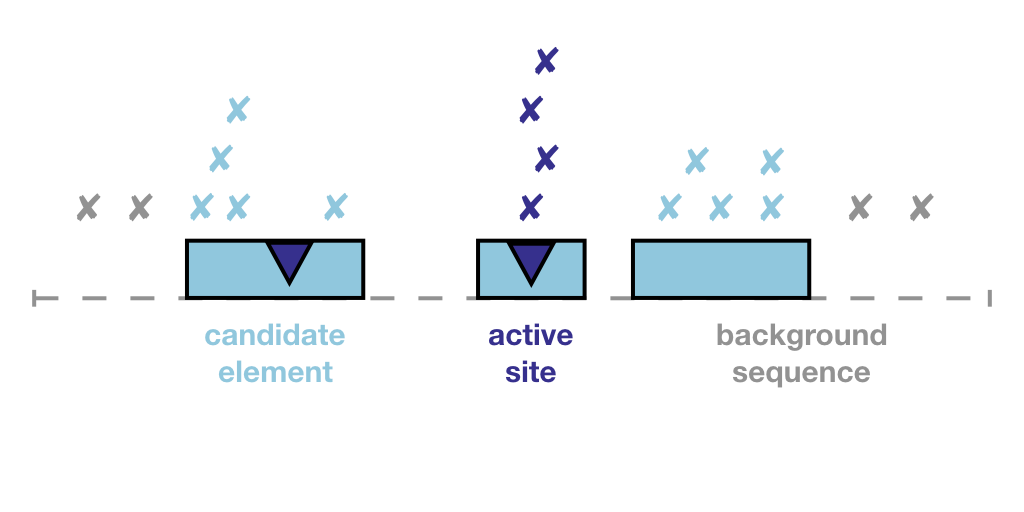
\includegraphics[width=0.75\linewidth]{ADWGS_diagram} \caption{The ActiveDriverWGS Model}\label{fig:pressure}
\end{figure}

\section{Input Data}\label{input-data}

ActiveDriverWGSR requires a file for somatic \texttt{mutations} and a
file for genomic \texttt{elements}. A third optional file for
\texttt{sites} can be specified by the user. Elements may contain
multiple segments but each element must have a unique ID.

\begin{verbatim}
library(ActiveDriverWGSR)

data("cll_mutations")
head(cll_mutations)
\end{verbatim}

\begin{verbatim}
##          chr      pos1      pos2 ref alt       patient  cc
## 779701  chr6  96651182  96651183  AA   T 001-0002-03TD CLL
## 779702 chr10 106556005 106556005   C   T 001-0002-03TD CLL
## 779703 chr10 107457352 107457352   C   T 001-0002-03TD CLL
## 779704 chr10 108111334 108111334   C   A 001-0002-03TD CLL
## 779705 chr10 109605024 109605024   T   A 001-0002-03TD CLL
##  [ reached getOption("max.print") -- omitted 1 row ]
\end{verbatim}

\begin{verbatim}
data("cancer_genes")
head(cancer_genes)
\end{verbatim}

\begin{verbatim}
##      chr   start     end       id
## 648 chr1 2488103 2488172 TNFRSF14
## 649 chr1 2489164 2489273 TNFRSF14
## 650 chr1 2489781 2489907 TNFRSF14
## 651 chr1 2491261 2491417 TNFRSF14
## 652 chr1 2492062 2492153 TNFRSF14
## 653 chr1 2492932 2492963 TNFRSF14
\end{verbatim}

\begin{verbatim}
data("cancer_gene_sites")
head(cancer_gene_sites)
\end{verbatim}

\begin{verbatim}
##         chr    start      end                  id
## 337831 chr1 11169412 11169412 MTOR NM_004958 2488
## 337834 chr1 11169413 11169413 MTOR NM_004958 2488
## 337837 chr1 11169414 11169414 MTOR NM_004958 2487
## 337839 chr1 11169415 11169415 MTOR NM_004958 2487
## 337841 chr1 11169416 11169416 MTOR NM_004958 2487
## 337843 chr1 11169418 11169418 MTOR NM_004958 2486
\end{verbatim}

\subsection{Importing BED12 Files as Input
Regions}\label{importing-bed12-files-as-input-regions}

For elements and sites written in BED12 files, the
prepare\_elements\_from\_BED12 function can be used to read the file and
adapt it to fulfill the format requirements for the \texttt{elements}
and \texttt{sites} parameters of the ActiveDriverWGS function. For more
information on the BED12 format, please refer to the
\href{https://genome.ucsc.edu/FAQ/FAQformat.html\#format1}{UCSC
guidelines}. In this example, elements are adapted from annotations for
protein coding genes from
\href{https://www.gencodegenes.org/human/release_19.html}{GENCODE.v19}
for chromosome 17.

\begin{verbatim}
elements = prepare_elements_from_BED12(
  system.file(
    "extdata", 
    "chr17.coding_regions.bed", 
    package = "ActiveDriverWGSR", 
    mustWork = TRUE))
\end{verbatim}

\begin{verbatim}
## 
##  1189  Rows :: Processing row 100  200  300  400  500  600  700  800  900  1000  1100  
##  Preparing Elements Complete 
##  RM 0 lines
\end{verbatim}

\begin{verbatim}
head(elements)
\end{verbatim}

\begin{verbatim}
##     chr starts  ends                                             id
## 1 chr17   6006  6168 gc19_pc.cds::gencode::DOC2B::ENSG00000272636.1
## 2 chr17  11205 11332 gc19_pc.cds::gencode::DOC2B::ENSG00000272636.1
## 3 chr17  11871 11981 gc19_pc.cds::gencode::DOC2B::ENSG00000272636.1
## 4 chr17  13920 13995 gc19_pc.cds::gencode::DOC2B::ENSG00000272636.1
## 5 chr17  22327 22407 gc19_pc.cds::gencode::DOC2B::ENSG00000272636.1
## 6 chr17  30897 31270 gc19_pc.cds::gencode::DOC2B::ENSG00000272636.1
\end{verbatim}

\section{Basic Use}\label{basic-use}

ActiveDriverWGS can be run simply with the mutations file, the elements
file and an optional sites file. In this example, mutations are adapted
from the \href{https://www.nature.com/articles/nature12477}{Alexandrov
et al, 2013} dataset for chronic lymphocytic leukemia (CLL) patients.
Regions are adapted from the
\href{https://cancer.sanger.ac.uk/census}{cancer gene census} and
annotations for protein coding genes are adapted from GENCODE.v19.

\begin{verbatim}
some_genes = c("ATM", "MYD88", "NOTCH1",
               "SF3B1", "XPO1", "SOCS1", 
               "CNOT3", "DDX3X", "KMT2A", 
               "HIF1A", "APC")

results = ActiveDriverWGS(mutations = cll_mutations,
                          elements = cancer_genes[cancer_genes$id %in% some_genes,],
                          sites = cancer_gene_sites)
\end{verbatim}

\begin{verbatim}
## 0 remove hypermut, n= 0 ,  0 %
## hypermuted samples:   
## 
## reversing 0 positions
## Removing  0  SNVs & indels in uninterpretable regions of the genome 
## 
## Tests to do:  11 
## ...........
\end{verbatim}

\subsection{Parameter Interpretation}\label{parameter-interpretation}

ActiveDriverWGS has several adjustable parameters:

\begin{enumerate}
\def\labelenumi{\arabic{enumi})}
\item
  \texttt{window\_size}: A narrow background window in which mutation
  rates are assumed to remain constant. We have optimized this parameter
  on the PCAWG dataset to be 50,000 bps for SNVs and indels.
\item
  \texttt{filter\_hyper\_MB}: The threshold for the number of simple
  somatic mutations per megabase above which a sample is considered
  hypermutated. We define the default to be 30 mutations/megabase
  according to published literature.
\item
  \texttt{recovery.dir}: The directory for writing recovery files for
  ActiveDriverWGS. If the directory does not exist, it will be created.
  If none is specified, ActiveDriverWGS will create the directory
  ActiveDriverWGS\_recovery.
\item
  \texttt{mc.cores}: The number of cores that the user wishes to
  allocate to running ActiveDriverWGS. For more information, refer to
  the R package
  \href{https://stat.ethz.ch/R-manual/R-devel/library/parallel/doc/parallel.pdf}{parallel}.
\end{enumerate}

\section{Interpreting the Results}\label{interpreting-the-results}

\begin{verbatim}
head(results)
\end{verbatim}

\begin{verbatim}
##       id  pp_element element_muts_obs element_muts_exp element_enriched
## 1    ATM 0.001807467                2                0             TRUE
## 2  MYD88 0.004976353                1                0             TRUE
##     pp_site site_muts_obs site_muts_exp site_enriched fdr_element fdr_site
## 1 1.0000000            NA            NA            NA  0.01241211        1
## 2 1.0000000            NA            NA            NA  0.01241211        1
##   has_site_mutations
## 1                   
## 2                   
##  [ reached getOption("max.print") -- omitted 4 rows ]
\end{verbatim}

ActiveDriverWGS will return results in a data frame format with the
following columns.

\begin{enumerate}
\def\labelenumi{\arabic{enumi})}
\item
  \texttt{id}: The identifier for the element.
\item
  \texttt{pp\_element}: The p-value associated with enrichment of
  mutations in the element.
\item
  \texttt{element\_muts\_obs}: Number of patients with mutations in the
  element.
\item
  \texttt{element\_muts\_exp}: Number of expected patients with
  mutations in the element.
\item
  \texttt{element\_enriched}: Boolean indicating whether an enrichment
  of mutations is observed.
\item
  \texttt{pp\_site}: The p-value associated with enrichment of mutations
  in the sites.
\item
  \texttt{site\_muts\_obs}: Number of patients with mutations in the
  sites.
\item
  \texttt{site\_enriched}: Expected number of patients with mutations in
  the sites.
\item
  \texttt{fdr\_element}: FDR corrected p-value associated with the
  element.
\item
  \texttt{fdr\_site}: FDR corrected p-value associated with the site.
\item
  \texttt{has\_site\_mutations}: ``V'' indicating the presence of site
  mutations
\end{enumerate}

\section{Adapting ActiveDriverWGS to
HPCCs}\label{adapting-activedriverwgs-to-hpccs}

Compute time increases linearly with the number of samples, mutations
and regions. Hence, the two main functions integral to ActiveDriverWGS
have also been made available in the public domain and can be adapted by
the user to their local high performance computing clusters.

\subsubsection{1. format\_muts}\label{format_muts}

This function formats the mutations data frame, removes hyper-mutated
samples and removes non-mitochondrial mutations in extrachromosomal
regions. It adds an additional column to the mutations data frame that
provides the trinucleotide context of the given mutation which will be
later used to estimate the mutational distribution across signatures.

\subsubsection{2. ADWGS\_test}\label{adwgs_test}

This function calculates the enrichment of mutations for a particular
region id. It applies a Poisson generalized linear regression model
across mutation signatures to identify enriched regions.

\subsection{Example}\label{example}

The following example demonstrates how to build an ActiveDriverWGS
pipeline which can be adapted to HPCCs. The idea is that the list of ids
can be split into manageable pieces and run in parallel jobs. Note that
the creation of GRanges objects is part of the ActiveDriverWGS wrapper
function and must be completed manually by users wishing to create
personalized pipelines. Also, note that multiple testing corrections
have be recalculated in additional steps.

\begin{verbatim}
library(GenomicRanges)

# Loading elements & creating a GRanges object
data(cancer_genes)
gr_element_coords = GRanges(seqnames = cancer_genes$chr,
                            IRanges(start = cancer_genes$start,
                                    end = cancer_genes$end),
                            mcols = cancer_genes$id)

# Loading sites & creating a GRanges object
data(cancer_gene_sites)
gr_site_coords = GRanges(seqnames = cancer_gene_sites$chr,
                         IRanges(start = cancer_gene_sites$start,
                                 end = cancer_gene_sites$end),
                         mocols = cancer_gene_sites$id)

# Loading mutations, format muts & creating a GRanges object
data(cll_mutations)

# format_muts
cll_mutations = format_muts(cll_mutations,
                            filter_hyper_MB = 30)
\end{verbatim}

\begin{verbatim}
## 0 remove hypermut, n= 0 ,  0 %
## hypermuted samples:   
## 
## reversing 0 positions
## Removing  0  SNVs & indels in uninterpretable regions of the genome
\end{verbatim}

\begin{verbatim}
gr_maf = GRanges(cll_mutations$chr,
                 IRanges(start = cll_mutations$pos1,
                         end = cll_mutations$pos2),
                 mcols=cll_mutations[,c("patient", "tag")])

# Examplifying the ATM Element
id = "ATM"

result = ADWGS_test(id = id,
                    gr_element_coords = gr_element_coords,
                    gr_site_coords = gr_site_coords,
                    gr_maf = gr_maf,
                    win_size = 50000)
\end{verbatim}

\begin{verbatim}
## .
\end{verbatim}

\begin{verbatim}
result
\end{verbatim}

\begin{verbatim}
##      id  pp_element element_muts_obs element_muts_exp element_enriched
## 95% ATM 0.001807467                2                0             TRUE
##     pp_site site_muts_obs site_muts_exp site_enriched
## 95%      NA            NA            NA            NA
\end{verbatim}


\end{document}
